\author{Patrick Bucher}
\title{px: PEAX Command Line Client}
\subtitle{Wirtschaftsprojekt, Herbstsemester 2019}
\date{\today}
\maketitle
\thispagestyle{empty}

\section*{Abstract}

Die vorliegende Arbeit handelt von der Software \texttt{px}, die den Zugriff auf die RESTful API von PEAX für Benutzer mit einem technischen Hintergrund erleichtern soll. PEAX ist ein digitaler Briefkasten, womit Endanwender ihre Post über verschiedene Kanäle empfangen und in einem komfortablen Web-Portal verwalten können.

Die Software \texttt{px} wurde auf Basis der \textsc{Unix}-Philosophie im Rahmen eines agilen Projekts als Kommandozeilenprogramm umgesetzt. Die Qualität der Software wird mithilfe einer Teststrategie sichergestellt, die zu einem grossen Teil auf Testskripts setzt.

Im Ergebnis vereinfacht \texttt{px} den \textit{direkten} Zugriff auf die RESTful API, d.h. ohne Verwendung des Webportals, indem die Handhabung von Zugriffstokens (Access Token, Refresh Token) abstrahiert wird, und dem Benutzer intuitiv bedienbare sowie generische, HTTP-nahe Befehle für das Ansteuern verschiedener Endpoints zur Verfügung gestellt werden.

Das Projektergebnis wird im Rahmen des PEAX-Ideation-Prozesses validiert und kann für verschiedene Anwendungszwecke im Zusammenhang mit dem PEAX-Portal eingesetzt und erweitert werden, was im Rahmen eines OpenSource-Projekts geschehen kann.

\vfill

\begin{multicols}{2}
    \begin{description}
        \item[Auftraggeber] \textsc{Pascal Meier}\\PEAX AG
        \item[Betreuer] \textsc{Roger Diehl}\\HSLU Informatik
        \item[Experte] \textsc{Roland Gisler}\\HSLU Informatik
    \end{description}
    \columnbreak
    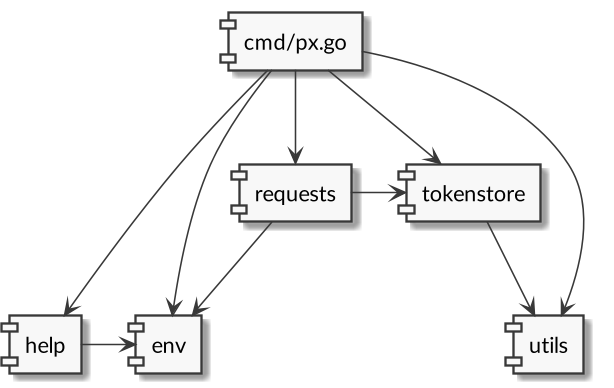
\includegraphics[width=\linewidth]{pics/title.png}
\end{multicols}
